% R4 — TextGuard v2 vs v1 on held-out domains (Energy, FNSPID). Framing approved by Aryan
% 2026-10-19. Every number is from results/summary_r4_*.csv and summary_r4_reading.json
% (python -m src.analyze_r4); figures paper/figures/r4_dss.pdf, r4_fbr.pdf (src/figures_r4.py).
% Pre-registration: PROJECT_STATUS §10g, commit 1e13815 (before any held-out output); v2 frozen as
% V3 in 0a58aba; Note 1 (Energy prompt label) 2a4fe25, a disclosure that changes no test. Runs
% verified in e675e9c (§7f) before any metric. Needs: booktabs. Fake texts are SYNTHETIC research
% artefacts (ethics, CLAUDE.md §14).

\subsection{Does a revised TextGuard generalise to held-out domains?}
\label{sec:r4}

\emph{Headline.} TextGuard~v2's protection against the forward-looking attack generalises to
held-out domains on Model~5, but its lower False Block Rate does not. Pooled over both held-out
domains, A2 moves the undefended forecast $+0.180\sigma$ toward the lie and $+0.021\sigma$ under
v2, a cut of 88\%, and v2 is lower than v1 ($+0.096\sigma$) by $0.075\sigma$ (Holm $p < 0.001$).
But v2 blocks 18.4\% of genuine reports against v1's 7.0\% (22.4\% on FNSPID), reversing the
ordering seen on validation (6.3\% vs 11.3\%). On our hand-labelled FNSPID headlines the judge
gives a direction to 11 of the 33 neutral ones while never reversing one, which points to the
cause. No improvement transfers to Qwen2.5-7B. Validation overstated v2, as we stated before the
test; the held-out test caught it. By our pre-registered rule the reading is \emph{v2 buys
protection at a cost (False Block Rate)}, not \emph{v2 improves on v1}.

\paragraph{Design.} TextGuard~v2 was developed and frozen on the original domains' validation
split only (judging every sentence or headline separately, checking each claim against evidence in
its own reference frame, and capping the text's effect at $1\sigma$). We then tested it once,
next to the frozen v1, clipping ($k = 0.5$), never\_trust, always\_trust and the output projection
of \emph{Market Signal Injection} % TODO P8: \citep{} key — not yet in references.bib
(anchor15: the forecast projected onto $\pm15\%$ of the last value, untuned), on two
domains no part of the system had seen: \textbf{Energy} (weekly U.S.\ retail gasoline, 665 windows,
352 with a report; an easy case, since its reports restate the target) and \textbf{FNSPID}
(10 S\&P~500 stocks, weekly closes, 1{,}031 windows, 1{,}006 with a bundle of that week's
Benzinga headlines; a hard case). Every text period is a test period. Targets: Model~5
(primary) and Qwen2.5-7B, re-run on Kaggle in one software setup per model. Attacks are the
rule-based flip and R3's A1 (selective flip), A2 (one appended forward-looking sentence) and A3
($\times10$ magnitude; Energy only), with 345\,/\,102\,/\,345\,/\,218 attacked Energy windows and
108\,/\,31\,/\,538 FNSPID windows. One Holm family per target ($m = 79$), smallest effects of
interest $0.05\sigma$ (DSS), 10\% FBR budget, 5\,pp FBR difference and 10\% real-text MSE were
fixed before any held-out output existed.

\paragraph{One disclosed wording error, found before any output was seen.}
Energy's prompt labels the all-grades series as regular gasoline, a wording error in our
pre-registration that contradicts our own data description: the target is the U.S.\ all-grades
weekly retail price, while the reports quote the regular-grade price. The gap is about \$0.09;
every comparison is paired within one prompt, so no pre-registered test can be biased by it.
Energy accuracy (MSE vs persistence) may be slightly affected and is noted where reported.

\begin{table}[t]
\centering\small
\caption{Held-out test, Model~5: DSS ($\sigma$, toward the lie), and the False Block Rate on
genuine reports. Verdicts by the pre-registered rules (Holm within the target's family of 79).
Pooled = both domains, equal window weight.}
\label{tab:r4}
\begin{tabular}{llrrrr}
\toprule
Cell & Attack & Undefended & TextGuard v1 & TextGuard v2 & Clip \\
\midrule
Energy & flip & $+0.045$ & $+0.022$ & $+0.018$ & $+0.043$ \\
       & A2   & $+0.061$ & $+0.055$ & $+0.027$ & $+0.059$ \\
       & A3   & $-0.002$ & $-0.001$ & $-0.001$ & $-0.002$ \\
FNSPID & flip & $+0.083$ & $+0.051$ & $+0.010$ & $+0.038$ \\
       & A2   & $+0.256$ & $+0.122$ & $+0.016$ & $+0.125$ \\
Pooled & flip & $+0.054$ & $+0.029$ & $+0.016$ & $+0.042$ \\
       & A1   & $+0.043$ & $+0.038$ & $+0.023$ & $+0.030$ \\
       & A2   & $+0.180$ & $+0.096$ & $+0.021$ & $+0.099$ \\
\midrule
\multicolumn{2}{l}{FBR Energy / FNSPID / pooled (\%)} & 0 & 1.1 / 9.0 / 7.0 & 7.1 / 22.4 / 18.4 & 0.3 / 13.6 / 10.2 \\
\bottomrule
\end{tabular}
\end{table}

\begin{figure}[t]
\centering
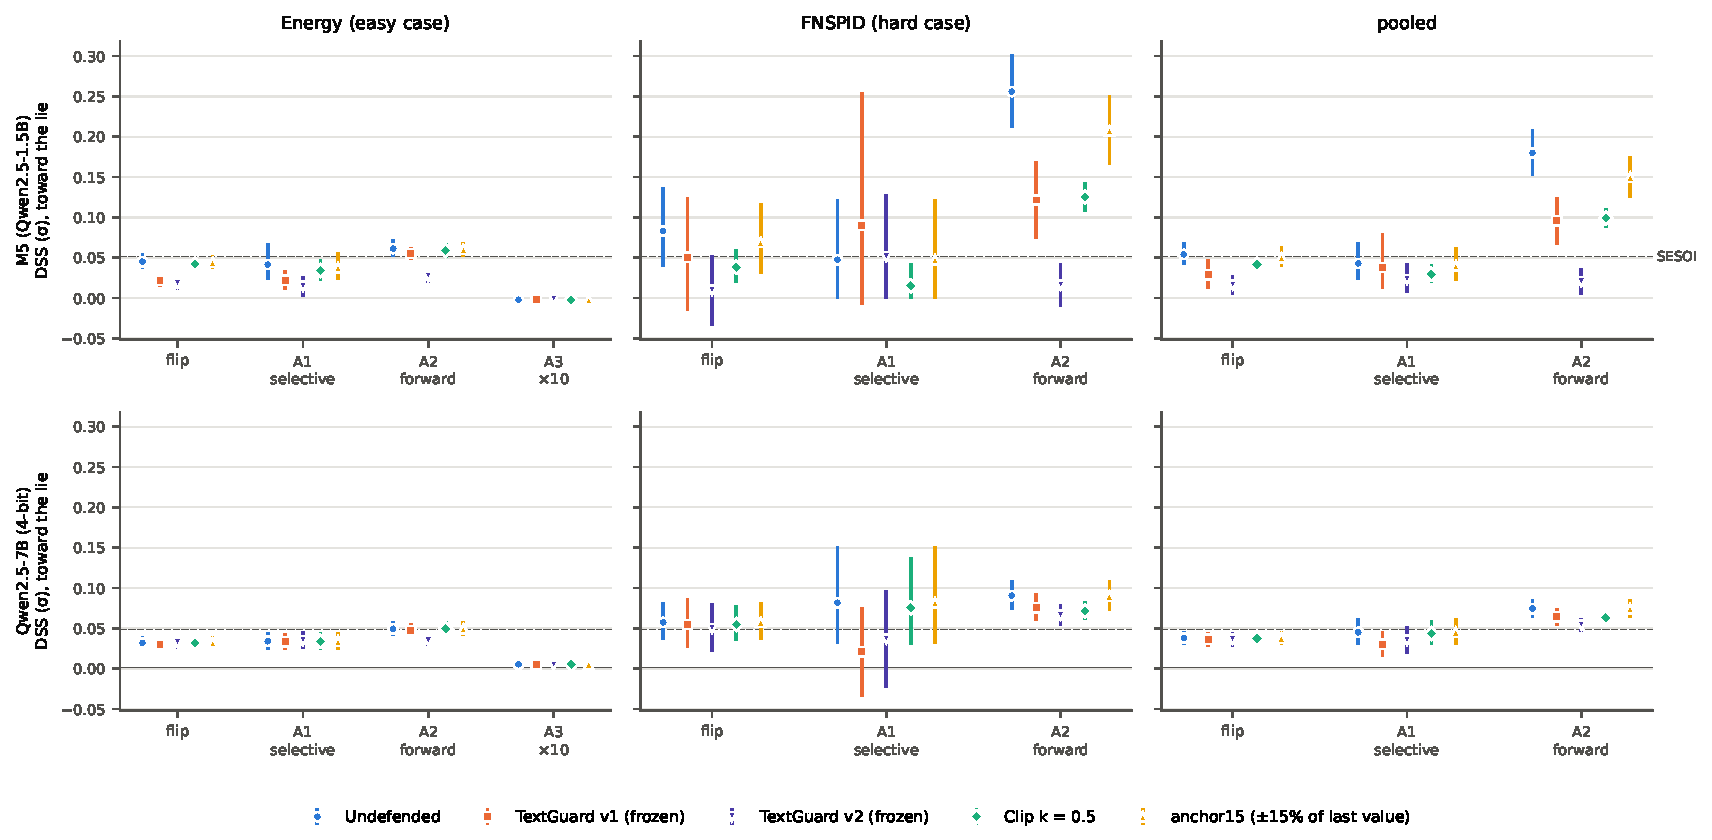
\includegraphics[width=\linewidth]{figures/r4_dss.pdf}
\caption{Held-out DSS under each attack, undefended and under each defence, for Model~5 (top) and
Qwen2.5-7B (bottom); Energy, FNSPID and pooled. Whiskers: 95\% bootstrap CI. Dashed line: smallest
effect of interest ($0.05\sigma$). A3 is run on Energy only.}
\label{fig:r4-dss}
\end{figure}

\begin{figure}[t]
\centering
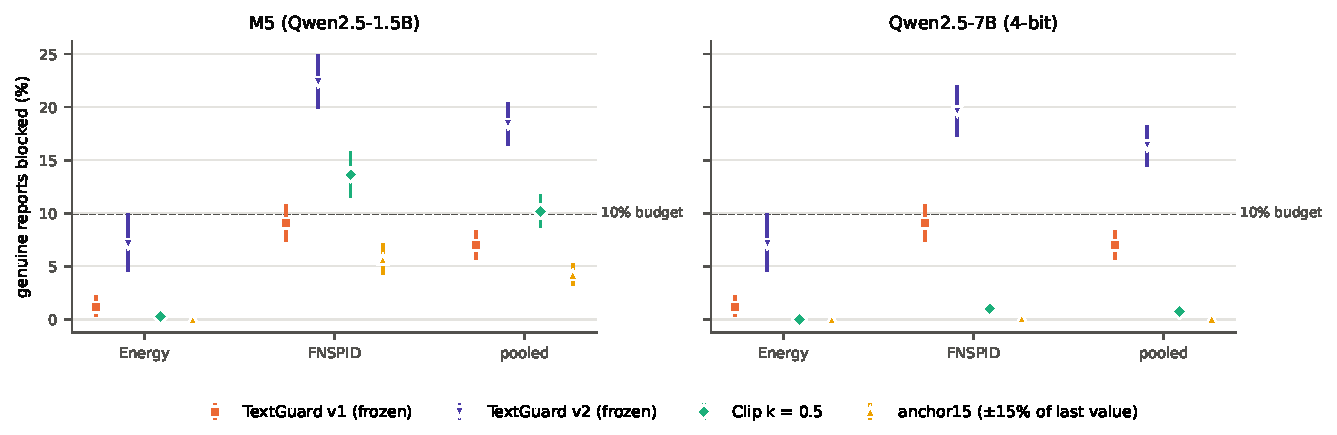
\includegraphics[width=\linewidth]{figures/r4_fbr.pdf}
\caption{False Block Rate on genuine held-out reports (applied weight $< 0.5$) per defence, with
95\% bootstrap CI. Dashed line: the pre-registered 10\% budget.}
\label{fig:r4-fbr}
\end{figure}

\paragraph{The attacks.} On Model~5 the flip is weaker on held-out data than on the original
domains: $+0.054\sigma$ pooled (CI $0.042$--$0.069$, ``fooled''), $+0.045\sigma$ on Energy (below
the SESOI) and $+0.083\sigma$ on FNSPID. A2 is the strongest attack, as in R3: $+0.180\sigma$
pooled, $+0.061\sigma$ on Energy and $+0.256\sigma$ on FNSPID. A1 is significant but below the
SESOI pooled, and A3 does not push ($-0.002\sigma$, bounded), as in R3. The medians of the
per-window DSS are 0 for the flip and A1: most windows do not move at all, and the means come from
a minority that do. Removing the single most extreme window changes no pooled mean by more than
$0.017\sigma$.

\paragraph{v2 against v1 and the other defences (Model~5).} \emph{A2:} v2 is lower than v1 on
FNSPID ($-0.105\sigma$) and pooled ($-0.075\sigma$), and lower than clipping by about the same
amount. Its residual, $+0.021\sigma$ pooled (CI $0.004$--$0.037$), lies entirely below the SESOI
but is significantly above zero (Holm $p < 0.001$). Our vocabulary, fixed before the test,
reserves ``bounded'' for estimates that are \emph{not} significant: ``A significant estimate below
the SESOI is reported as `significant but negligible'. A non-rejection is `bounded below the
SESOI' only if the whole 95\% CI lies inside $\pm$SESOI''; a defence ``stops'' an attack only if
the defended DSS is bounded, and a reduction whose residual is inconclusive or negligible reads
``reduces; residual not shown to be below the SESOI''. That is the label v2 receives on A2: a
small, measurable residual, not a stop. The per-sentence split does the work: v2's judge read
A2's appended sentence in the claimed direction in 345/345 Energy and 538/538 FNSPID texts, and
the cap alone (gate switched off) leaves A2 at $+0.133\sigma$. v1's whole-report judge read the
genuine past claim on Energy (99.4\% opposite to the lie, so v1 is \emph{evaded} there, as
predicted), but on FNSPID's short headline bundles it read the appended sentence in 54\% of texts,
which is why v1 also reduces A2 there. \emph{Flip and A1:} pooled, both versions reduce DSS by
less than the SESOI. On FNSPID, v2 reduces the flip by $0.073\sigma$ (to $+0.010\sigma$; residual
not shown to be below the SESOI) and v1 does not; on FNSPID's 31 A1 windows v1 reads $+0.090\sigma$
against $+0.048\sigma$ undefended (no change shown; mostly Merck). v2 and v1 do not differ by
$0.05\sigma$ on any flip or A1 cell. \emph{anchor15} binds more often
than we expected on FNSPID (it blocks 5.7\% of genuine bundles) yet barely reduces A2
($+0.150\sigma$ pooled). never\_trust has DSS 0 and blocks every report.

\paragraph{The cost: blocked genuine reports.} The prediction stated before the test was that v2
might miss the budget on FNSPID, because a bundle averages 9.6 judged units (headlines or their
sentences) and the gate takes the minimum over all of them. It does: v2 blocks 22.4\% of genuine
FNSPID bundles (v1 9.0\%) and 7.1\% of genuine Energy reports (v1 1.1\%); pooled 18.4\% vs 7.0\%,
a difference of $+11.4$\,pp (exact McNemar, Holm $p < 0.001$). Validation's ordering (v2 6.3\% vs
v1 11.3\%) is reversed. Most of it is the gate, not the cap: without the cap v2 still blocks
16.3\% pooled; the cap alone blocks 3.3\%. The judge check below locates the source: spurious
directions read into neutral headlines, each of which the minimum gate can turn into a block
when the weak weekly trend disagrees. Clipping is just over budget (10.2\%) on Model~5, because
Model~5's genuine reactions to headlines exceed $0.5\sigma$ in 13.6\% of FNSPID windows.

\paragraph{Accuracy.} Genuine FNSPID headlines make Model~5 \emph{less} accurate: its MSE is
$1.06\sigma^2$ with them and $0.48\sigma^2$ without them (persistence $0.32\sigma^2$). Any defence
that damps the text therefore helps here, and v2's real-text MSE is lower than v1's
($-0.249\sigma^2$ pooled) and than the undefended model's. This gain partly reflects damping
harmful text rather than v2's claim checking: the cap alone gives $0.66\sigma^2$ on FNSPID. On
Energy, v2 and v1 are within $\pm10\%$. Model~5 is also less accurate on Energy with the report
than without it ($0.024$ vs $0.011\sigma^2$; persistence $0.007$), the cell the disclosure above
may affect: the reports' regular-grade price is on average \$0.092 below the series, and Model~5's
mean error shifts down with the report (from $+\$0.013$ to $-\$0.018$), in the direction of the
lower quoted price; it copies the quoted price exactly in only 2.8\% of windows (exploratory check,
not pre-registered).

\paragraph{Qwen2.5-7B.} The larger model is pushed less (flip $+0.038\sigma$ pooled, below the
SESOI) but is fooled on FNSPID by the flip ($+0.057\sigma$), A1 ($+0.082\sigma$) and A2
($+0.090\sigma$), and by A2 pooled ($+0.074\sigma$). Neither version helps: A2 stays fooled under
v1 ($+0.064\sigma$) and v2 ($+0.054\sigma$), so both are \emph{evaded} on Qwen2.5-7B, and v2 still
blocks 16.3\% of genuine reports (v1 7.0\%). Its accuracy is unchanged by either. The reading is
\emph{no improvement over v1 shown}.

\paragraph{The pre-registered decision rules, read mechanically.} Model~5 pooled: \emph{v2 buys
protection at a cost (FBR)}: it is lower than v1 on A2 by more than the SESOI, worse on no attack,
not less accurate, but over the FBR budget and significantly above v1. \emph{v2 closes R3's A2
gap}: not met, because on the pooled held-out data v1 is no longer evaded by A2 (it reduces it,
via FNSPID). On Energy, where v1 \emph{is} evaded, v2 lowers A2 by $0.034\sigma$, which is below
the SESOI. Energy alone: \emph{no improvement over v1 shown}; FNSPID alone: \emph{protection at a
cost}. Qwen2.5-7B: \emph{no improvement over v1 shown} in every cell. FBR budget: v1 meets it in
every cell; v2 only on Energy; clipping on Energy and (Qwen2.5-7B) everywhere.

\paragraph{Judge checks.} On our 50 hand-labelled FNSPID headlines (34\% directional), v2's
change answer agrees with the label on 76\% ($\kappa = 0.60$; an always-``none'' rater would score
66\%). It never reverses a direction and finds 16 of the 17 directional headlines, but it gives a
direction to 11 of the 33 headlines labelled neutral. After v2's confidence floor the agreement is
80\% (3 neutral headlines still get a direction, 8 directional ones are dropped). The outlook
answer agrees on 60\%. v1 cannot be scored on these labels (it judges whole bundles; one labelled
headline is a bundle on its own). On genuine FNSPID text v1 answers ``none'' for 31\% of bundles
and v2 for 46\% of headlines. This comparison was added at the author's request after the runs;
it was not pre-registered.

\paragraph{Robustness (pre-stated, descriptive).} \emph{Semantic mismatch:} without the FNSPID flip
bundles whose edited headline keeps a causal connector (52 of 108), the undefended flip on FNSPID
stays at $+0.072\sigma$ (from $+0.083\sigma$); the A1 effect on FNSPID disappears ($+0.006\sigma$,
18 windows), so the small A1 effect there lives in the flagged bundles. \emph{COVID:} without
February--May 2020 every Model~5 reading is unchanged; v2's FBR is 16.3\% pooled. \emph{FNSPID with
a 10-year $\sigma$:} DSS shrinks (A2 pooled $+0.107\sigma$ undefended), several cells drop below
the SESOI, v1 becomes \emph{evaded} by A2 pooled, and v2 is still lower than v1 on FNSPID A2 and
blocks 12.3\% pooled (v1 3.5\%). \emph{Ablations:} the as-built v2 (V0, without the validation fix)
behaves like the frozen V3 here (FBR 19.7\%, A2 $+0.021\sigma$); without the cap, A2 is
$-0.013\sigma$ but real-text MSE rises to $0.85\sigma^2$ on FNSPID. \emph{Scan:} including the one
excluded flip text changes no reading. \emph{Memorisation:} no target $\times$ domain is flagged
(at most 4 unexplained exact matches, none above the placebo rate; FNSPID prices compared to the
cent, since its stored closes carry float noise beyond two decimals). \emph{Per stock (A1):} 1--6
windows per stock; Merck's 4 windows carry most of Model~5's A1 effect on FNSPID.

\paragraph{What this shows and what it does not.} Judging each sentence on its own, frozen on
validation, transfers to unseen domains as a defence against an appended forward-looking lie on
the model that follows such a sentence most (Model~5). It does not transfer the validation-set
False Block Rate: on headline bundles the judge reads directions into neutral headlines, more
units means more chances that one of them disagrees with a weak trend, and the minimum gate then
blocks the bundle. It does not help the larger model. Validation overstated v2, as stated before
the test, and the held-out test is what showed it.
